% Created by tikzDevice version 0.6.2-92-0ad2792 on 2013-03-12 19:48:03
% !TEX encoding = UTF-8 Unicode
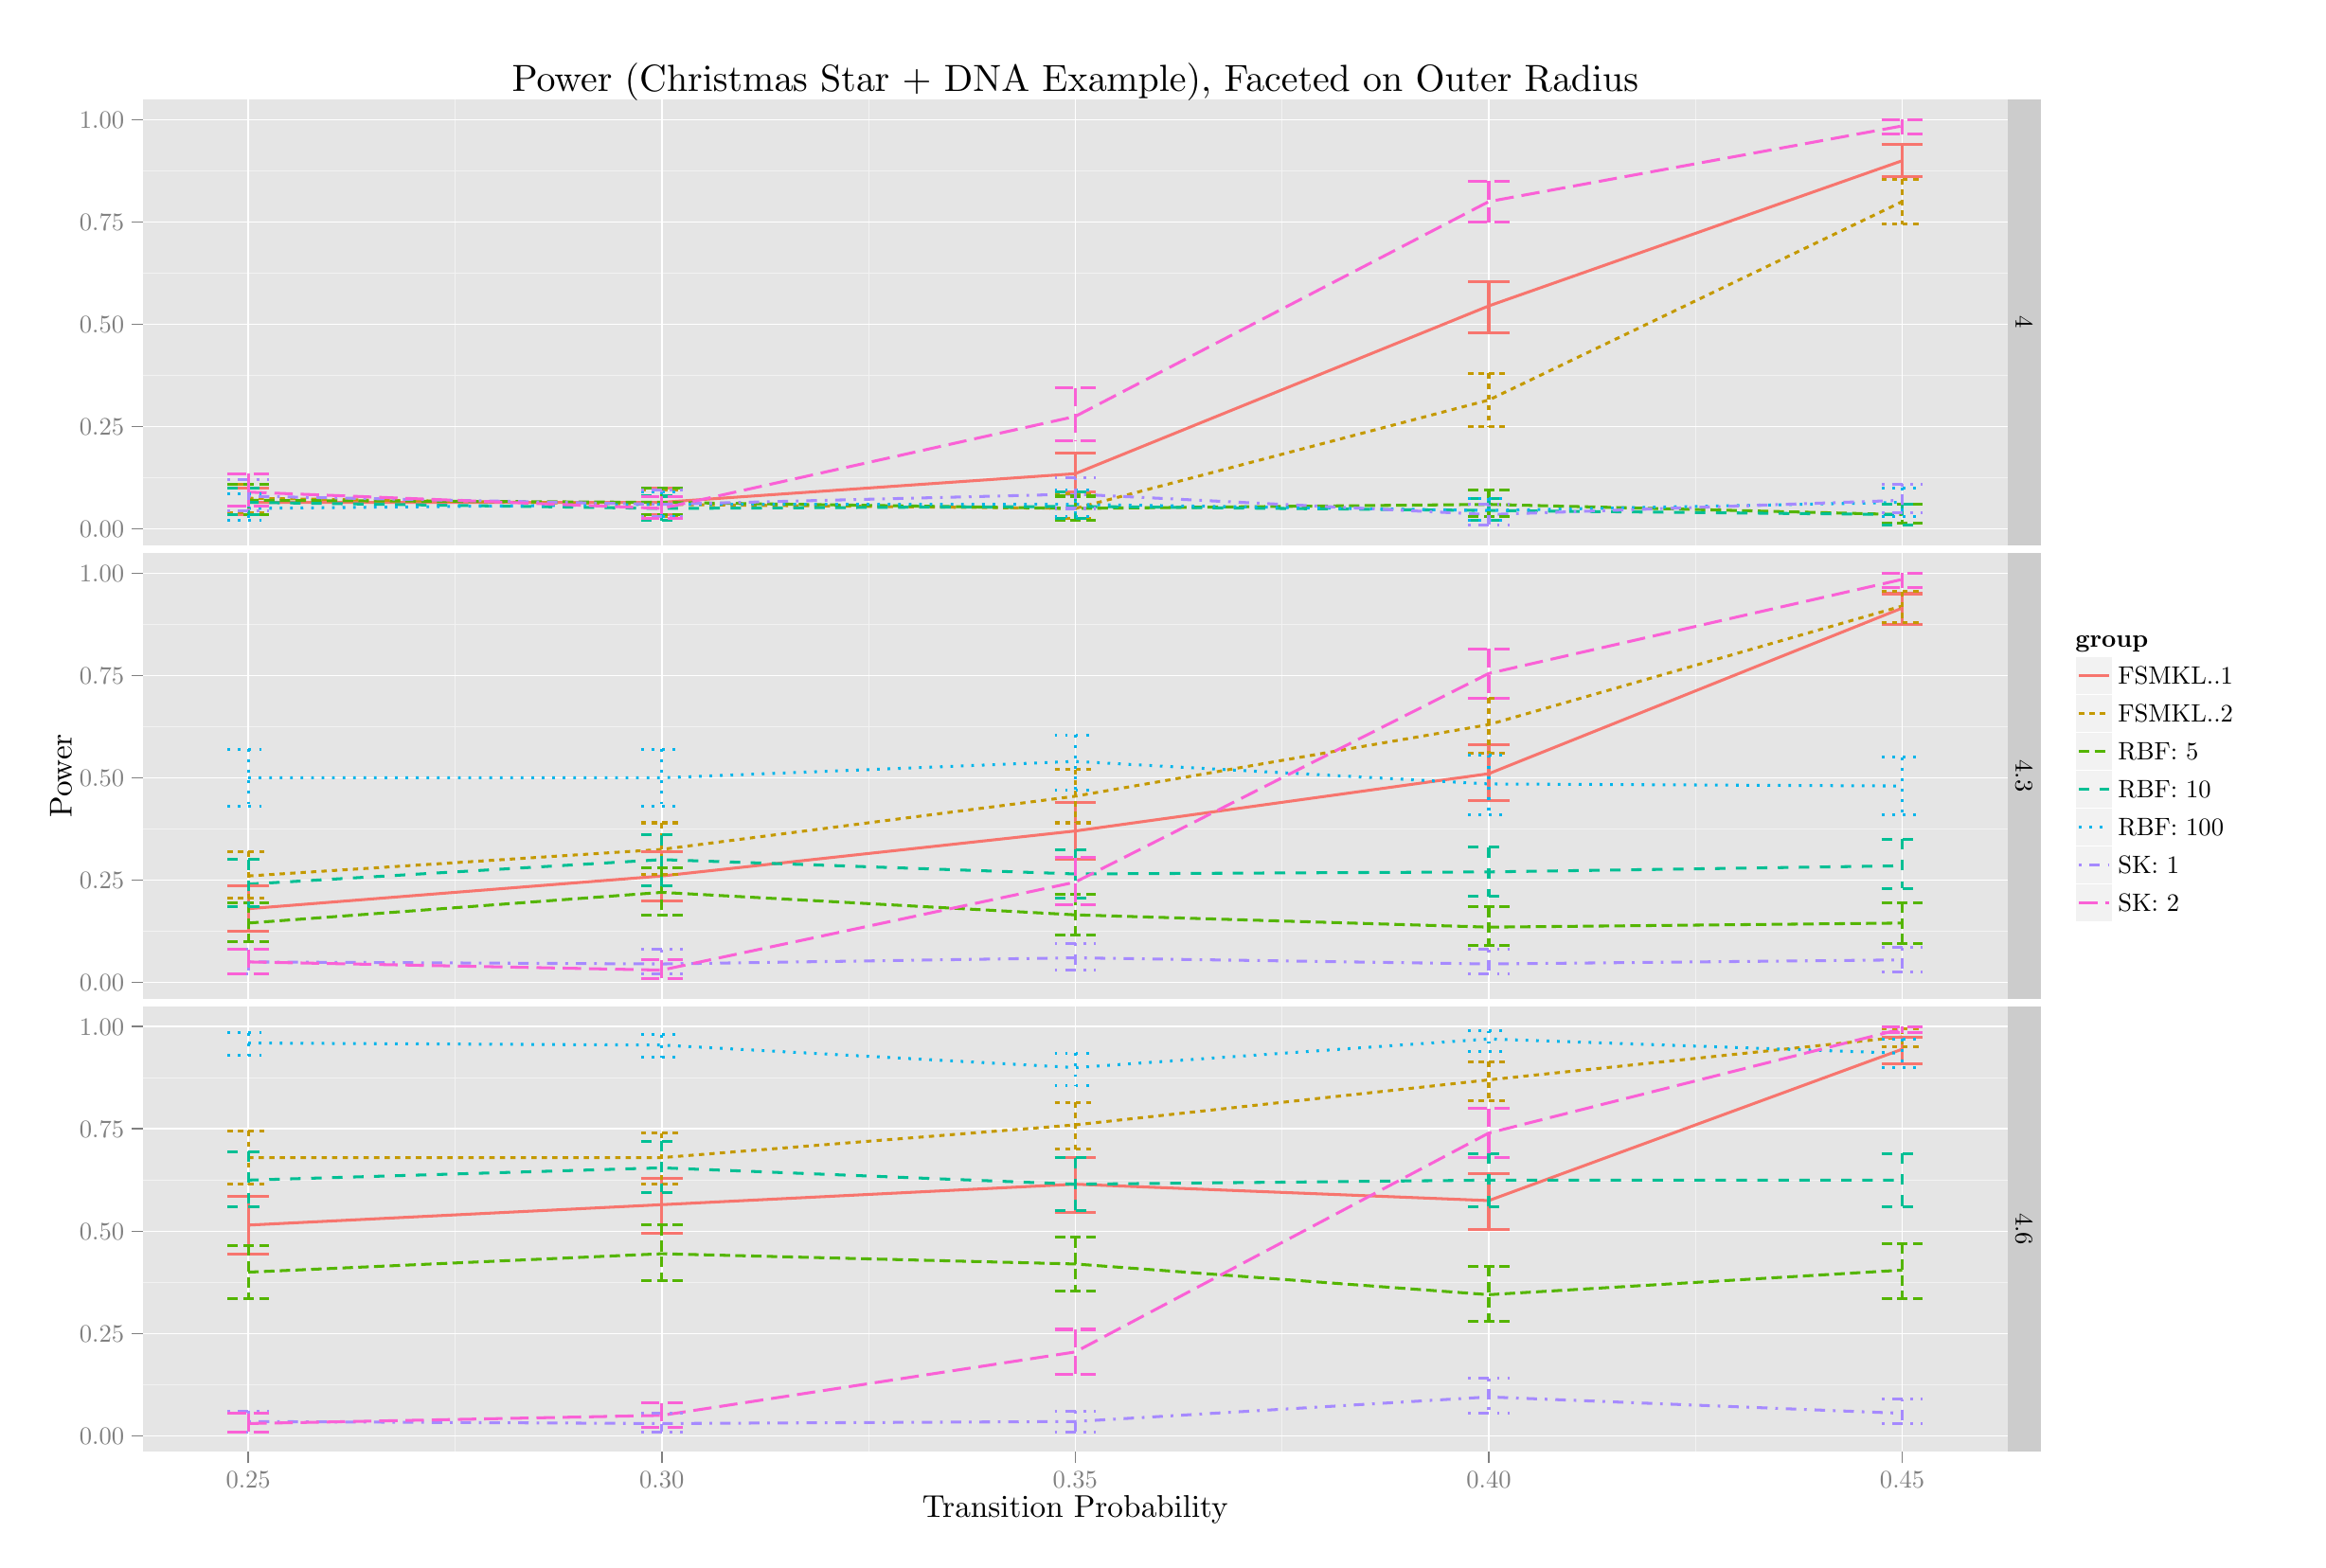
\begin{tikzpicture}[x=1pt,y=1pt]
\definecolor[named]{fillColor}{rgb}{1.00,1.00,1.00}
\path[use as bounding box,fill=fillColor,fill opacity=0.00] (0,0) rectangle (867.24,578.16);
\begin{scope}
\path[clip] (  0.00,  0.00) rectangle (867.24,578.16);
\definecolor[named]{drawColor}{rgb}{1.00,1.00,1.00}
\definecolor[named]{fillColor}{rgb}{1.00,1.00,1.00}

\path[draw=drawColor,line width= 0.6pt,line join=round,line cap=round,fill=fillColor] ( -0.00, -0.00) rectangle (867.24,578.16);
\end{scope}
\begin{scope}
\path[clip] ( 44.49,380.14) rectangle (756.04,550.17);
\definecolor[named]{fillColor}{rgb}{0.90,0.90,0.90}

\path[fill=fillColor] ( 44.49,380.14) rectangle (756.04,550.17);
\definecolor[named]{drawColor}{rgb}{0.95,0.95,0.95}

\path[draw=drawColor,line width= 0.3pt,line join=round] ( 44.49,405.82) --
	(756.04,405.82);

\path[draw=drawColor,line width= 0.3pt,line join=round] ( 44.49,444.86) --
	(756.04,444.86);

\path[draw=drawColor,line width= 0.3pt,line join=round] ( 44.49,483.89) --
	(756.04,483.89);

\path[draw=drawColor,line width= 0.3pt,line join=round] ( 44.49,522.93) --
	(756.04,522.93);

\path[draw=drawColor,line width= 0.3pt,line join=round] (163.60,380.14) --
	(163.60,550.17);

\path[draw=drawColor,line width= 0.3pt,line join=round] (321.38,380.14) --
	(321.38,550.17);

\path[draw=drawColor,line width= 0.3pt,line join=round] (479.15,380.14) --
	(479.15,550.17);

\path[draw=drawColor,line width= 0.3pt,line join=round] (636.92,380.14) --
	(636.92,550.17);
\definecolor[named]{drawColor}{rgb}{1.00,1.00,1.00}

\path[draw=drawColor,line width= 0.6pt,line join=round] ( 44.49,386.30) --
	(756.04,386.30);

\path[draw=drawColor,line width= 0.6pt,line join=round] ( 44.49,425.34) --
	(756.04,425.34);

\path[draw=drawColor,line width= 0.6pt,line join=round] ( 44.49,464.37) --
	(756.04,464.37);

\path[draw=drawColor,line width= 0.6pt,line join=round] ( 44.49,503.41) --
	(756.04,503.41);

\path[draw=drawColor,line width= 0.6pt,line join=round] ( 44.49,542.45) --
	(756.04,542.45);

\path[draw=drawColor,line width= 0.6pt,line join=round] ( 84.72,380.14) --
	( 84.72,550.17);

\path[draw=drawColor,line width= 0.6pt,line join=round] (242.49,380.14) --
	(242.49,550.17);

\path[draw=drawColor,line width= 0.6pt,line join=round] (400.26,380.14) --
	(400.26,550.17);

\path[draw=drawColor,line width= 0.6pt,line join=round] (558.03,380.14) --
	(558.03,550.17);

\path[draw=drawColor,line width= 0.6pt,line join=round] (715.81,380.14) --
	(715.81,550.17);
\definecolor[named]{drawColor}{rgb}{0.97,0.46,0.43}

\path[draw=drawColor,line width= 1.1pt,line join=round] ( 84.72,396.45) --
	(242.49,396.45) --
	(400.26,407.38) --
	(558.03,471.40) --
	(715.81,526.83);
\definecolor[named]{drawColor}{rgb}{0.77,0.60,0.00}

\path[draw=drawColor,line width= 1.1pt,dash pattern=on 2pt off 2pt ,line join=round] ( 84.72,398.01) --
	(242.49,395.67) --
	(400.26,394.11) --
	(558.03,435.49) --
	(715.81,511.22);
\definecolor[named]{drawColor}{rgb}{0.33,0.71,0.00}

\path[draw=drawColor,line width= 1.1pt,dash pattern=on 4pt off 2pt ,line join=round] ( 84.72,397.23) --
	(242.49,396.45) --
	(400.26,394.11) --
	(558.03,395.67) --
	(715.81,391.77);
\definecolor[named]{drawColor}{rgb}{0.00,0.75,0.58}

\path[draw=drawColor,line width= 1.1pt,dash pattern=on 4pt off 4pt ,line join=round] ( 84.72,396.45) --
	(242.49,394.11) --
	(400.26,394.89) --
	(558.03,393.33) --
	(715.81,391.77);
\definecolor[named]{drawColor}{rgb}{0.00,0.71,0.92}

\path[draw=drawColor,line width= 1.1pt,dash pattern=on 1pt off 3pt ,line join=round] ( 84.72,394.11) --
	(242.49,395.67) --
	(400.26,395.67) --
	(558.03,393.33) --
	(715.81,396.45);
\definecolor[named]{drawColor}{rgb}{0.65,0.54,1.00}

\path[draw=drawColor,line width= 1.1pt,dash pattern=on 1pt off 3pt on 4pt off 3pt ,line join=round] ( 84.72,398.79) --
	(242.49,395.67) --
	(400.26,399.58) --
	(558.03,391.77) --
	(715.81,397.23);
\definecolor[named]{drawColor}{rgb}{0.98,0.38,0.84}

\path[draw=drawColor,line width= 1.1pt,dash pattern=on 7pt off 3pt ,line join=round] ( 84.72,400.36) --
	(242.49,394.11) --
	(400.26,429.24) --
	(558.03,511.22) --
	(715.81,540.10);
\definecolor[named]{drawColor}{rgb}{0.97,0.46,0.43}

\path[draw=drawColor,line width= 1.1pt,line join=round] ( 76.83,401.92) --
	( 92.61,401.92);

\path[draw=drawColor,line width= 1.1pt,line join=round] ( 84.72,401.92) --
	( 84.72,391.77);

\path[draw=drawColor,line width= 1.1pt,line join=round] ( 76.83,391.77) --
	( 92.61,391.77);

\path[draw=drawColor,line width= 1.1pt,line join=round] (234.60,401.92) --
	(250.38,401.92);

\path[draw=drawColor,line width= 1.1pt,line join=round] (242.49,401.92) --
	(242.49,391.77);

\path[draw=drawColor,line width= 1.1pt,line join=round] (234.60,391.77) --
	(250.38,391.77);

\path[draw=drawColor,line width= 1.1pt,line join=round] (392.37,415.19) --
	(408.15,415.19);

\path[draw=drawColor,line width= 1.1pt,line join=round] (400.26,415.19) --
	(400.26,400.36);

\path[draw=drawColor,line width= 1.1pt,line join=round] (392.37,400.36) --
	(408.15,400.36);

\path[draw=drawColor,line width= 1.1pt,line join=round] (550.15,480.77) --
	(565.92,480.77);

\path[draw=drawColor,line width= 1.1pt,line join=round] (558.03,480.77) --
	(558.03,461.23);

\path[draw=drawColor,line width= 1.1pt,line join=round] (550.15,461.23) --
	(565.92,461.23);

\path[draw=drawColor,line width= 1.1pt,line join=round] (707.92,533.08) --
	(723.70,533.08);

\path[draw=drawColor,line width= 1.1pt,line join=round] (715.81,533.08) --
	(715.81,520.59);

\path[draw=drawColor,line width= 1.1pt,line join=round] (707.92,520.59) --
	(723.70,520.59);
\definecolor[named]{drawColor}{rgb}{0.77,0.60,0.00}

\path[draw=drawColor,line width= 1.1pt,dash pattern=on 2pt off 2pt ,line join=round] ( 76.83,403.48) --
	( 92.61,403.48);

\path[draw=drawColor,line width= 1.1pt,dash pattern=on 2pt off 2pt ,line join=round] ( 84.72,403.48) --
	( 84.72,392.55);

\path[draw=drawColor,line width= 1.1pt,dash pattern=on 2pt off 2pt ,line join=round] ( 76.83,392.55) --
	( 92.61,392.55);

\path[draw=drawColor,line width= 1.1pt,dash pattern=on 2pt off 2pt ,line join=round] (234.60,401.14) --
	(250.38,401.14);

\path[draw=drawColor,line width= 1.1pt,dash pattern=on 2pt off 2pt ,line join=round] (242.49,401.14) --
	(242.49,390.99);

\path[draw=drawColor,line width= 1.1pt,dash pattern=on 2pt off 2pt ,line join=round] (234.60,390.99) --
	(250.38,390.99);

\path[draw=drawColor,line width= 1.1pt,dash pattern=on 2pt off 2pt ,line join=round] (392.37,399.58) --
	(408.15,399.58);

\path[draw=drawColor,line width= 1.1pt,dash pattern=on 2pt off 2pt ,line join=round] (400.26,399.58) --
	(400.26,390.21);

\path[draw=drawColor,line width= 1.1pt,dash pattern=on 2pt off 2pt ,line join=round] (392.37,390.21) --
	(408.15,390.21);

\path[draw=drawColor,line width= 1.1pt,dash pattern=on 2pt off 2pt ,line join=round] (550.15,445.64) --
	(565.92,445.64);

\path[draw=drawColor,line width= 1.1pt,dash pattern=on 2pt off 2pt ,line join=round] (558.03,445.64) --
	(558.03,425.34);

\path[draw=drawColor,line width= 1.1pt,dash pattern=on 2pt off 2pt ,line join=round] (550.15,425.34) --
	(565.92,425.34);

\path[draw=drawColor,line width= 1.1pt,dash pattern=on 2pt off 2pt ,line join=round] (707.92,519.81) --
	(723.70,519.81);

\path[draw=drawColor,line width= 1.1pt,dash pattern=on 2pt off 2pt ,line join=round] (715.81,519.81) --
	(715.81,502.63);

\path[draw=drawColor,line width= 1.1pt,dash pattern=on 2pt off 2pt ,line join=round] (707.92,502.63) --
	(723.70,502.63);
\definecolor[named]{drawColor}{rgb}{0.33,0.71,0.00}

\path[draw=drawColor,line width= 1.1pt,dash pattern=on 4pt off 2pt ,line join=round] ( 76.83,403.48) --
	( 92.61,403.48);

\path[draw=drawColor,line width= 1.1pt,dash pattern=on 4pt off 2pt ,line join=round] ( 84.72,403.48) --
	( 84.72,391.77);

\path[draw=drawColor,line width= 1.1pt,dash pattern=on 4pt off 2pt ,line join=round] ( 76.83,391.77) --
	( 92.61,391.77);

\path[draw=drawColor,line width= 1.1pt,dash pattern=on 4pt off 2pt ,line join=round] (234.60,401.92) --
	(250.38,401.92);

\path[draw=drawColor,line width= 1.1pt,dash pattern=on 4pt off 2pt ,line join=round] (242.49,401.92) --
	(242.49,391.77);

\path[draw=drawColor,line width= 1.1pt,dash pattern=on 4pt off 2pt ,line join=round] (234.60,391.77) --
	(250.38,391.77);

\path[draw=drawColor,line width= 1.1pt,dash pattern=on 4pt off 2pt ,line join=round] (392.37,398.81) --
	(408.15,398.81);

\path[draw=drawColor,line width= 1.1pt,dash pattern=on 4pt off 2pt ,line join=round] (400.26,398.81) --
	(400.26,389.43);

\path[draw=drawColor,line width= 1.1pt,dash pattern=on 4pt off 2pt ,line join=round] (392.37,389.43) --
	(408.15,389.43);

\path[draw=drawColor,line width= 1.1pt,dash pattern=on 4pt off 2pt ,line join=round] (550.15,401.16) --
	(565.92,401.16);

\path[draw=drawColor,line width= 1.1pt,dash pattern=on 4pt off 2pt ,line join=round] (558.03,401.16) --
	(558.03,390.99);

\path[draw=drawColor,line width= 1.1pt,dash pattern=on 4pt off 2pt ,line join=round] (550.15,390.99) --
	(565.92,390.99);

\path[draw=drawColor,line width= 1.1pt,dash pattern=on 4pt off 2pt ,line join=round] (707.92,395.67) --
	(723.70,395.67);

\path[draw=drawColor,line width= 1.1pt,dash pattern=on 4pt off 2pt ,line join=round] (715.81,395.67) --
	(715.81,388.63);

\path[draw=drawColor,line width= 1.1pt,dash pattern=on 4pt off 2pt ,line join=round] (707.92,388.63) --
	(723.70,388.63);
\definecolor[named]{drawColor}{rgb}{0.00,0.75,0.58}

\path[draw=drawColor,line width= 1.1pt,dash pattern=on 4pt off 4pt ,line join=round] ( 76.83,401.92) --
	( 92.61,401.92);

\path[draw=drawColor,line width= 1.1pt,dash pattern=on 4pt off 4pt ,line join=round] ( 84.72,401.92) --
	( 84.72,391.77);

\path[draw=drawColor,line width= 1.1pt,dash pattern=on 4pt off 4pt ,line join=round] ( 76.83,391.77) --
	( 92.61,391.77);

\path[draw=drawColor,line width= 1.1pt,dash pattern=on 4pt off 4pt ,line join=round] (234.60,398.81) --
	(250.38,398.81);

\path[draw=drawColor,line width= 1.1pt,dash pattern=on 4pt off 4pt ,line join=round] (242.49,398.81) --
	(242.49,389.43);

\path[draw=drawColor,line width= 1.1pt,dash pattern=on 4pt off 4pt ,line join=round] (234.60,389.43) --
	(250.38,389.43);

\path[draw=drawColor,line width= 1.1pt,dash pattern=on 4pt off 4pt ,line join=round] (392.37,400.36) --
	(408.15,400.36);

\path[draw=drawColor,line width= 1.1pt,dash pattern=on 4pt off 4pt ,line join=round] (400.26,400.36) --
	(400.26,390.21);

\path[draw=drawColor,line width= 1.1pt,dash pattern=on 4pt off 4pt ,line join=round] (392.37,390.21) --
	(408.15,390.21);

\path[draw=drawColor,line width= 1.1pt,dash pattern=on 4pt off 4pt ,line join=round] (550.15,398.01) --
	(565.92,398.01);

\path[draw=drawColor,line width= 1.1pt,dash pattern=on 4pt off 4pt ,line join=round] (558.03,398.01) --
	(558.03,389.43);

\path[draw=drawColor,line width= 1.1pt,dash pattern=on 4pt off 4pt ,line join=round] (550.15,389.43) --
	(565.92,389.43);

\path[draw=drawColor,line width= 1.1pt,dash pattern=on 4pt off 4pt ,line join=round] (707.92,395.67) --
	(723.70,395.67);

\path[draw=drawColor,line width= 1.1pt,dash pattern=on 4pt off 4pt ,line join=round] (715.81,395.67) --
	(715.81,387.86);

\path[draw=drawColor,line width= 1.1pt,dash pattern=on 4pt off 4pt ,line join=round] (707.92,387.86) --
	(723.70,387.86);
\definecolor[named]{drawColor}{rgb}{0.00,0.71,0.92}

\path[draw=drawColor,line width= 1.1pt,dash pattern=on 1pt off 3pt ,line join=round] ( 76.83,399.58) --
	( 92.61,399.58);

\path[draw=drawColor,line width= 1.1pt,dash pattern=on 1pt off 3pt ,line join=round] ( 84.72,399.58) --
	( 84.72,389.43);

\path[draw=drawColor,line width= 1.1pt,dash pattern=on 1pt off 3pt ,line join=round] ( 76.83,389.43) --
	( 92.61,389.43);

\path[draw=drawColor,line width= 1.1pt,dash pattern=on 1pt off 3pt ,line join=round] (234.60,400.36) --
	(250.38,400.36);

\path[draw=drawColor,line width= 1.1pt,dash pattern=on 1pt off 3pt ,line join=round] (242.49,400.36) --
	(242.49,390.99);

\path[draw=drawColor,line width= 1.1pt,dash pattern=on 1pt off 3pt ,line join=round] (234.60,390.99) --
	(250.38,390.99);

\path[draw=drawColor,line width= 1.1pt,dash pattern=on 1pt off 3pt ,line join=round] (392.37,401.16) --
	(408.15,401.16);

\path[draw=drawColor,line width= 1.1pt,dash pattern=on 1pt off 3pt ,line join=round] (400.26,401.16) --
	(400.26,390.99);

\path[draw=drawColor,line width= 1.1pt,dash pattern=on 1pt off 3pt ,line join=round] (392.37,390.99) --
	(408.15,390.99);

\path[draw=drawColor,line width= 1.1pt,dash pattern=on 1pt off 3pt ,line join=round] (550.15,398.01) --
	(565.92,398.01);

\path[draw=drawColor,line width= 1.1pt,dash pattern=on 1pt off 3pt ,line join=round] (558.03,398.01) --
	(558.03,389.43);

\path[draw=drawColor,line width= 1.1pt,dash pattern=on 1pt off 3pt ,line join=round] (550.15,389.43) --
	(565.92,389.43);

\path[draw=drawColor,line width= 1.1pt,dash pattern=on 1pt off 3pt ,line join=round] (707.92,401.94) --
	(723.70,401.94);

\path[draw=drawColor,line width= 1.1pt,dash pattern=on 1pt off 3pt ,line join=round] (715.81,401.94) --
	(715.81,390.99);

\path[draw=drawColor,line width= 1.1pt,dash pattern=on 1pt off 3pt ,line join=round] (707.92,390.99) --
	(723.70,390.99);
\definecolor[named]{drawColor}{rgb}{0.65,0.54,1.00}

\path[draw=drawColor,line width= 1.1pt,dash pattern=on 1pt off 3pt on 4pt off 3pt ,line join=round] ( 76.83,405.04) --
	( 92.61,405.04);

\path[draw=drawColor,line width= 1.1pt,dash pattern=on 1pt off 3pt on 4pt off 3pt ,line join=round] ( 84.72,405.04) --
	( 84.72,393.33);

\path[draw=drawColor,line width= 1.1pt,dash pattern=on 1pt off 3pt on 4pt off 3pt ,line join=round] ( 76.83,393.33) --
	( 92.61,393.33);

\path[draw=drawColor,line width= 1.1pt,dash pattern=on 1pt off 3pt on 4pt off 3pt ,line join=round] (234.60,401.14) --
	(250.38,401.14);

\path[draw=drawColor,line width= 1.1pt,dash pattern=on 1pt off 3pt on 4pt off 3pt ,line join=round] (242.49,401.14) --
	(242.49,390.99);

\path[draw=drawColor,line width= 1.1pt,dash pattern=on 1pt off 3pt on 4pt off 3pt ,line join=round] (234.60,390.99) --
	(250.38,390.99);

\path[draw=drawColor,line width= 1.1pt,dash pattern=on 1pt off 3pt on 4pt off 3pt ,line join=round] (392.37,405.82) --
	(408.15,405.82);

\path[draw=drawColor,line width= 1.1pt,dash pattern=on 1pt off 3pt on 4pt off 3pt ,line join=round] (400.26,405.82) --
	(400.26,394.11);

\path[draw=drawColor,line width= 1.1pt,dash pattern=on 1pt off 3pt on 4pt off 3pt ,line join=round] (392.37,394.11) --
	(408.15,394.11);

\path[draw=drawColor,line width= 1.1pt,dash pattern=on 1pt off 3pt on 4pt off 3pt ,line join=round] (550.15,395.67) --
	(565.92,395.67);

\path[draw=drawColor,line width= 1.1pt,dash pattern=on 1pt off 3pt on 4pt off 3pt ,line join=round] (558.03,395.67) --
	(558.03,387.86);

\path[draw=drawColor,line width= 1.1pt,dash pattern=on 1pt off 3pt on 4pt off 3pt ,line join=round] (550.15,387.86) --
	(565.92,387.86);

\path[draw=drawColor,line width= 1.1pt,dash pattern=on 1pt off 3pt on 4pt off 3pt ,line join=round] (707.92,403.48) --
	(723.70,403.48);

\path[draw=drawColor,line width= 1.1pt,dash pattern=on 1pt off 3pt on 4pt off 3pt ,line join=round] (715.81,403.48) --
	(715.81,392.55);

\path[draw=drawColor,line width= 1.1pt,dash pattern=on 1pt off 3pt on 4pt off 3pt ,line join=round] (707.92,392.55) --
	(723.70,392.55);
\definecolor[named]{drawColor}{rgb}{0.98,0.38,0.84}

\path[draw=drawColor,line width= 1.1pt,dash pattern=on 7pt off 3pt ,line join=round] ( 76.83,407.38) --
	( 92.61,407.38);

\path[draw=drawColor,line width= 1.1pt,dash pattern=on 7pt off 3pt ,line join=round] ( 84.72,407.38) --
	( 84.72,394.89);

\path[draw=drawColor,line width= 1.1pt,dash pattern=on 7pt off 3pt ,line join=round] ( 76.83,394.89) --
	( 92.61,394.89);

\path[draw=drawColor,line width= 1.1pt,dash pattern=on 7pt off 3pt ,line join=round] (234.60,398.79) --
	(250.38,398.79);

\path[draw=drawColor,line width= 1.1pt,dash pattern=on 7pt off 3pt ,line join=round] (242.49,398.79) --
	(242.49,390.21);

\path[draw=drawColor,line width= 1.1pt,dash pattern=on 7pt off 3pt ,line join=round] (234.60,390.21) --
	(250.38,390.21);

\path[draw=drawColor,line width= 1.1pt,dash pattern=on 7pt off 3pt ,line join=round] (392.37,440.17) --
	(408.15,440.17);

\path[draw=drawColor,line width= 1.1pt,dash pattern=on 7pt off 3pt ,line join=round] (400.26,440.17) --
	(400.26,419.87);

\path[draw=drawColor,line width= 1.1pt,dash pattern=on 7pt off 3pt ,line join=round] (392.37,419.87) --
	(408.15,419.87);

\path[draw=drawColor,line width= 1.1pt,dash pattern=on 7pt off 3pt ,line join=round] (550.15,519.04) --
	(565.92,519.04);

\path[draw=drawColor,line width= 1.1pt,dash pattern=on 7pt off 3pt ,line join=round] (558.03,519.04) --
	(558.03,503.41);

\path[draw=drawColor,line width= 1.1pt,dash pattern=on 7pt off 3pt ,line join=round] (550.15,503.41) --
	(565.92,503.41);

\path[draw=drawColor,line width= 1.1pt,dash pattern=on 7pt off 3pt ,line join=round] (707.92,542.45) --
	(723.70,542.45);

\path[draw=drawColor,line width= 1.1pt,dash pattern=on 7pt off 3pt ,line join=round] (715.81,542.45) --
	(715.81,536.98);

\path[draw=drawColor,line width= 1.1pt,dash pattern=on 7pt off 3pt ,line join=round] (707.92,536.98) --
	(723.70,536.98);
\end{scope}
\begin{scope}
\path[clip] ( 44.49,207.09) rectangle (756.04,377.12);
\definecolor[named]{fillColor}{rgb}{0.90,0.90,0.90}

\path[fill=fillColor] ( 44.49,207.09) rectangle (756.04,377.12);
\definecolor[named]{drawColor}{rgb}{0.95,0.95,0.95}

\path[draw=drawColor,line width= 0.3pt,line join=round] ( 44.49,232.77) --
	(756.04,232.77);

\path[draw=drawColor,line width= 0.3pt,line join=round] ( 44.49,271.81) --
	(756.04,271.81);

\path[draw=drawColor,line width= 0.3pt,line join=round] ( 44.49,310.84) --
	(756.04,310.84);

\path[draw=drawColor,line width= 0.3pt,line join=round] ( 44.49,349.88) --
	(756.04,349.88);

\path[draw=drawColor,line width= 0.3pt,line join=round] (163.60,207.09) --
	(163.60,377.12);

\path[draw=drawColor,line width= 0.3pt,line join=round] (321.38,207.09) --
	(321.38,377.12);

\path[draw=drawColor,line width= 0.3pt,line join=round] (479.15,207.09) --
	(479.15,377.12);

\path[draw=drawColor,line width= 0.3pt,line join=round] (636.92,207.09) --
	(636.92,377.12);
\definecolor[named]{drawColor}{rgb}{1.00,1.00,1.00}

\path[draw=drawColor,line width= 0.6pt,line join=round] ( 44.49,213.25) --
	(756.04,213.25);

\path[draw=drawColor,line width= 0.6pt,line join=round] ( 44.49,252.29) --
	(756.04,252.29);

\path[draw=drawColor,line width= 0.6pt,line join=round] ( 44.49,291.32) --
	(756.04,291.32);

\path[draw=drawColor,line width= 0.6pt,line join=round] ( 44.49,330.36) --
	(756.04,330.36);

\path[draw=drawColor,line width= 0.6pt,line join=round] ( 44.49,369.40) --
	(756.04,369.40);

\path[draw=drawColor,line width= 0.6pt,line join=round] ( 84.72,207.09) --
	( 84.72,377.12);

\path[draw=drawColor,line width= 0.6pt,line join=round] (242.49,207.09) --
	(242.49,377.12);

\path[draw=drawColor,line width= 0.6pt,line join=round] (400.26,207.09) --
	(400.26,377.12);

\path[draw=drawColor,line width= 0.6pt,line join=round] (558.03,207.09) --
	(558.03,377.12);

\path[draw=drawColor,line width= 0.6pt,line join=round] (715.81,207.09) --
	(715.81,377.12);
\definecolor[named]{drawColor}{rgb}{0.97,0.46,0.43}

\path[draw=drawColor,line width= 1.1pt,line join=round] ( 84.72,241.36) --
	(242.49,253.85) --
	(400.26,271.03) --
	(558.03,292.89) --
	(715.81,356.12);
\definecolor[named]{drawColor}{rgb}{0.77,0.60,0.00}

\path[draw=drawColor,line width= 1.1pt,dash pattern=on 2pt off 2pt ,line join=round] ( 84.72,253.85) --
	(242.49,264.00) --
	(400.26,284.30) --
	(558.03,311.62) --
	(715.81,356.90);
\definecolor[named]{drawColor}{rgb}{0.33,0.71,0.00}

\path[draw=drawColor,line width= 1.1pt,dash pattern=on 4pt off 2pt ,line join=round] ( 84.72,235.89) --
	(242.49,247.60) --
	(400.26,239.02) --
	(558.03,234.33) --
	(715.81,235.89);
\definecolor[named]{drawColor}{rgb}{0.00,0.75,0.58}

\path[draw=drawColor,line width= 1.1pt,dash pattern=on 4pt off 4pt ,line join=round] ( 84.72,250.73) --
	(242.49,260.10) --
	(400.26,254.63) --
	(558.03,255.41) --
	(715.81,257.75);
\definecolor[named]{drawColor}{rgb}{0.00,0.71,0.92}

\path[draw=drawColor,line width= 1.1pt,dash pattern=on 1pt off 3pt ,line join=round] ( 84.72,291.32) --
	(242.49,291.32) --
	(400.26,297.57) --
	(558.03,288.98) --
	(715.81,288.20);
\definecolor[named]{drawColor}{rgb}{0.65,0.54,1.00}

\path[draw=drawColor,line width= 1.1pt,dash pattern=on 1pt off 3pt on 4pt off 3pt ,line join=round] ( 84.72,221.06) --
	(242.49,220.28) --
	(400.26,222.62) --
	(558.03,220.28) --
	(715.81,221.84);
\definecolor[named]{drawColor}{rgb}{0.98,0.38,0.84}

\path[draw=drawColor,line width= 1.1pt,dash pattern=on 7pt off 3pt ,line join=round] ( 84.72,221.06) --
	(242.49,217.94) --
	(400.26,251.51) --
	(558.03,331.14) --
	(715.81,367.05);
\definecolor[named]{drawColor}{rgb}{0.97,0.46,0.43}

\path[draw=drawColor,line width= 1.1pt,line join=round] ( 76.83,249.97) --
	( 92.61,249.97);

\path[draw=drawColor,line width= 1.1pt,line join=round] ( 84.72,249.97) --
	( 84.72,232.77);

\path[draw=drawColor,line width= 1.1pt,line join=round] ( 76.83,232.77) --
	( 92.61,232.77);

\path[draw=drawColor,line width= 1.1pt,line join=round] (234.60,263.22) --
	(250.38,263.22);

\path[draw=drawColor,line width= 1.1pt,line join=round] (242.49,263.22) --
	(242.49,244.48);

\path[draw=drawColor,line width= 1.1pt,line join=round] (234.60,244.48) --
	(250.38,244.48);

\path[draw=drawColor,line width= 1.1pt,line join=round] (392.37,281.96) --
	(408.15,281.96);

\path[draw=drawColor,line width= 1.1pt,line join=round] (400.26,281.96) --
	(400.26,260.10);

\path[draw=drawColor,line width= 1.1pt,line join=round] (392.37,260.10) --
	(408.15,260.10);

\path[draw=drawColor,line width= 1.1pt,line join=round] (550.15,303.82) --
	(565.92,303.82);

\path[draw=drawColor,line width= 1.1pt,line join=round] (558.03,303.82) --
	(558.03,282.74);

\path[draw=drawColor,line width= 1.1pt,line join=round] (550.15,282.74) --
	(565.92,282.74);

\path[draw=drawColor,line width= 1.1pt,line join=round] (707.92,361.59) --
	(723.70,361.59);

\path[draw=drawColor,line width= 1.1pt,line join=round] (715.81,361.59) --
	(715.81,349.88);

\path[draw=drawColor,line width= 1.1pt,line join=round] (707.92,349.88) --
	(723.70,349.88);
\definecolor[named]{drawColor}{rgb}{0.77,0.60,0.00}

\path[draw=drawColor,line width= 1.1pt,dash pattern=on 2pt off 2pt ,line join=round] ( 76.83,263.22) --
	( 92.61,263.22);

\path[draw=drawColor,line width= 1.1pt,dash pattern=on 2pt off 2pt ,line join=round] ( 84.72,263.22) --
	( 84.72,245.26);

\path[draw=drawColor,line width= 1.1pt,dash pattern=on 2pt off 2pt ,line join=round] ( 76.83,245.26) --
	( 92.61,245.26);

\path[draw=drawColor,line width= 1.1pt,dash pattern=on 2pt off 2pt ,line join=round] (234.60,274.15) --
	(250.38,274.15);

\path[draw=drawColor,line width= 1.1pt,dash pattern=on 2pt off 2pt ,line join=round] (242.49,274.15) --
	(242.49,254.61);

\path[draw=drawColor,line width= 1.1pt,dash pattern=on 2pt off 2pt ,line join=round] (234.60,254.61) --
	(250.38,254.61);

\path[draw=drawColor,line width= 1.1pt,dash pattern=on 2pt off 2pt ,line join=round] (392.37,294.45) --
	(408.15,294.45);

\path[draw=drawColor,line width= 1.1pt,dash pattern=on 2pt off 2pt ,line join=round] (400.26,294.45) --
	(400.26,274.15);

\path[draw=drawColor,line width= 1.1pt,dash pattern=on 2pt off 2pt ,line join=round] (392.37,274.15) --
	(408.15,274.15);

\path[draw=drawColor,line width= 1.1pt,dash pattern=on 2pt off 2pt ,line join=round] (550.15,321.77) --
	(565.92,321.77);

\path[draw=drawColor,line width= 1.1pt,dash pattern=on 2pt off 2pt ,line join=round] (558.03,321.77) --
	(558.03,300.69);

\path[draw=drawColor,line width= 1.1pt,dash pattern=on 2pt off 2pt ,line join=round] (550.15,300.69) --
	(565.92,300.69);

\path[draw=drawColor,line width= 1.1pt,dash pattern=on 2pt off 2pt ,line join=round] (707.92,362.37) --
	(723.70,362.37);

\path[draw=drawColor,line width= 1.1pt,dash pattern=on 2pt off 2pt ,line join=round] (715.81,362.37) --
	(715.81,350.64);

\path[draw=drawColor,line width= 1.1pt,dash pattern=on 2pt off 2pt ,line join=round] (707.92,350.64) --
	(723.70,350.64);
\definecolor[named]{drawColor}{rgb}{0.33,0.71,0.00}

\path[draw=drawColor,line width= 1.1pt,dash pattern=on 4pt off 2pt ,line join=round] ( 76.83,243.70) --
	( 92.61,243.70);

\path[draw=drawColor,line width= 1.1pt,dash pattern=on 4pt off 2pt ,line join=round] ( 84.72,243.70) --
	( 84.72,228.87);

\path[draw=drawColor,line width= 1.1pt,dash pattern=on 4pt off 2pt ,line join=round] ( 76.83,228.87) --
	( 92.61,228.87);

\path[draw=drawColor,line width= 1.1pt,dash pattern=on 4pt off 2pt ,line join=round] (234.60,256.99) --
	(250.38,256.99);

\path[draw=drawColor,line width= 1.1pt,dash pattern=on 4pt off 2pt ,line join=round] (242.49,256.99) --
	(242.49,239.02);

\path[draw=drawColor,line width= 1.1pt,dash pattern=on 4pt off 2pt ,line join=round] (234.60,239.02) --
	(250.38,239.02);

\path[draw=drawColor,line width= 1.1pt,dash pattern=on 4pt off 2pt ,line join=round] (392.37,246.82) --
	(408.15,246.82);

\path[draw=drawColor,line width= 1.1pt,dash pattern=on 4pt off 2pt ,line join=round] (400.26,246.82) --
	(400.26,231.19);

\path[draw=drawColor,line width= 1.1pt,dash pattern=on 4pt off 2pt ,line join=round] (392.37,231.19) --
	(408.15,231.19);

\path[draw=drawColor,line width= 1.1pt,dash pattern=on 4pt off 2pt ,line join=round] (550.15,242.14) --
	(565.92,242.14);

\path[draw=drawColor,line width= 1.1pt,dash pattern=on 4pt off 2pt ,line join=round] (558.03,242.14) --
	(558.03,227.31);

\path[draw=drawColor,line width= 1.1pt,dash pattern=on 4pt off 2pt ,line join=round] (550.15,227.31) --
	(565.92,227.31);

\path[draw=drawColor,line width= 1.1pt,dash pattern=on 4pt off 2pt ,line join=round] (707.92,243.70) --
	(723.70,243.70);

\path[draw=drawColor,line width= 1.1pt,dash pattern=on 4pt off 2pt ,line join=round] (715.81,243.70) --
	(715.81,228.09);

\path[draw=drawColor,line width= 1.1pt,dash pattern=on 4pt off 2pt ,line join=round] (707.92,228.09) --
	(723.70,228.09);
\definecolor[named]{drawColor}{rgb}{0.00,0.75,0.58}

\path[draw=drawColor,line width= 1.1pt,dash pattern=on 4pt off 4pt ,line join=round] ( 76.83,260.10) --
	( 92.61,260.10);

\path[draw=drawColor,line width= 1.1pt,dash pattern=on 4pt off 4pt ,line join=round] ( 84.72,260.10) --
	( 84.72,242.14);

\path[draw=drawColor,line width= 1.1pt,dash pattern=on 4pt off 4pt ,line join=round] ( 76.83,242.14) --
	( 92.61,242.14);

\path[draw=drawColor,line width= 1.1pt,dash pattern=on 4pt off 4pt ,line join=round] (234.60,269.46) --
	(250.38,269.46);

\path[draw=drawColor,line width= 1.1pt,dash pattern=on 4pt off 4pt ,line join=round] (242.49,269.46) --
	(242.49,249.95);

\path[draw=drawColor,line width= 1.1pt,dash pattern=on 4pt off 4pt ,line join=round] (234.60,249.95) --
	(250.38,249.95);

\path[draw=drawColor,line width= 1.1pt,dash pattern=on 4pt off 4pt ,line join=round] (392.37,264.00) --
	(408.15,264.00);

\path[draw=drawColor,line width= 1.1pt,dash pattern=on 4pt off 4pt ,line join=round] (400.26,264.00) --
	(400.26,245.26);

\path[draw=drawColor,line width= 1.1pt,dash pattern=on 4pt off 4pt ,line join=round] (392.37,245.26) --
	(408.15,245.26);

\path[draw=drawColor,line width= 1.1pt,dash pattern=on 4pt off 4pt ,line join=round] (550.15,264.78) --
	(565.92,264.78);

\path[draw=drawColor,line width= 1.1pt,dash pattern=on 4pt off 4pt ,line join=round] (558.03,264.78) --
	(558.03,246.04);

\path[draw=drawColor,line width= 1.1pt,dash pattern=on 4pt off 4pt ,line join=round] (550.15,246.04) --
	(565.92,246.04);

\path[draw=drawColor,line width= 1.1pt,dash pattern=on 4pt off 4pt ,line join=round] (707.92,267.90) --
	(723.70,267.90);

\path[draw=drawColor,line width= 1.1pt,dash pattern=on 4pt off 4pt ,line join=round] (715.81,267.90) --
	(715.81,249.17);

\path[draw=drawColor,line width= 1.1pt,dash pattern=on 4pt off 4pt ,line join=round] (707.92,249.17) --
	(723.70,249.17);
\definecolor[named]{drawColor}{rgb}{0.00,0.71,0.92}

\path[draw=drawColor,line width= 1.1pt,dash pattern=on 1pt off 3pt ,line join=round] ( 76.83,302.25) --
	( 92.61,302.25);

\path[draw=drawColor,line width= 1.1pt,dash pattern=on 1pt off 3pt ,line join=round] ( 84.72,302.25) --
	( 84.72,280.39);

\path[draw=drawColor,line width= 1.1pt,dash pattern=on 1pt off 3pt ,line join=round] ( 76.83,280.39) --
	( 92.61,280.39);

\path[draw=drawColor,line width= 1.1pt,dash pattern=on 1pt off 3pt ,line join=round] (234.60,302.25) --
	(250.38,302.25);

\path[draw=drawColor,line width= 1.1pt,dash pattern=on 1pt off 3pt ,line join=round] (242.49,302.25) --
	(242.49,280.39);

\path[draw=drawColor,line width= 1.1pt,dash pattern=on 1pt off 3pt ,line join=round] (234.60,280.39) --
	(250.38,280.39);

\path[draw=drawColor,line width= 1.1pt,dash pattern=on 1pt off 3pt ,line join=round] (392.37,307.72) --
	(408.15,307.72);

\path[draw=drawColor,line width= 1.1pt,dash pattern=on 1pt off 3pt ,line join=round] (400.26,307.72) --
	(400.26,286.64);

\path[draw=drawColor,line width= 1.1pt,dash pattern=on 1pt off 3pt ,line join=round] (392.37,286.64) --
	(408.15,286.64);

\path[draw=drawColor,line width= 1.1pt,dash pattern=on 1pt off 3pt ,line join=round] (550.15,299.91) --
	(565.92,299.91);

\path[draw=drawColor,line width= 1.1pt,dash pattern=on 1pt off 3pt ,line join=round] (558.03,299.91) --
	(558.03,277.27);

\path[draw=drawColor,line width= 1.1pt,dash pattern=on 1pt off 3pt ,line join=round] (550.15,277.27) --
	(565.92,277.27);

\path[draw=drawColor,line width= 1.1pt,dash pattern=on 1pt off 3pt ,line join=round] (707.92,299.13) --
	(723.70,299.13);

\path[draw=drawColor,line width= 1.1pt,dash pattern=on 1pt off 3pt ,line join=round] (715.81,299.13) --
	(715.81,277.27);

\path[draw=drawColor,line width= 1.1pt,dash pattern=on 1pt off 3pt ,line join=round] (707.92,277.27) --
	(723.70,277.27);
\definecolor[named]{drawColor}{rgb}{0.65,0.54,1.00}

\path[draw=drawColor,line width= 1.1pt,dash pattern=on 1pt off 3pt on 4pt off 3pt ,line join=round] ( 76.83,225.74) --
	( 92.61,225.74);

\path[draw=drawColor,line width= 1.1pt,dash pattern=on 1pt off 3pt on 4pt off 3pt ,line join=round] ( 84.72,225.74) --
	( 84.72,216.38);

\path[draw=drawColor,line width= 1.1pt,dash pattern=on 1pt off 3pt on 4pt off 3pt ,line join=round] ( 76.83,216.38) --
	( 92.61,216.38);

\path[draw=drawColor,line width= 1.1pt,dash pattern=on 1pt off 3pt on 4pt off 3pt ,line join=round] (234.60,225.74) --
	(250.38,225.74);

\path[draw=drawColor,line width= 1.1pt,dash pattern=on 1pt off 3pt on 4pt off 3pt ,line join=round] (242.49,225.74) --
	(242.49,216.38);

\path[draw=drawColor,line width= 1.1pt,dash pattern=on 1pt off 3pt on 4pt off 3pt ,line join=round] (234.60,216.38) --
	(250.38,216.38);

\path[draw=drawColor,line width= 1.1pt,dash pattern=on 1pt off 3pt on 4pt off 3pt ,line join=round] (392.37,228.09) --
	(408.15,228.09);

\path[draw=drawColor,line width= 1.1pt,dash pattern=on 1pt off 3pt on 4pt off 3pt ,line join=round] (400.26,228.09) --
	(400.26,217.94);

\path[draw=drawColor,line width= 1.1pt,dash pattern=on 1pt off 3pt on 4pt off 3pt ,line join=round] (392.37,217.94) --
	(408.15,217.94);

\path[draw=drawColor,line width= 1.1pt,dash pattern=on 1pt off 3pt on 4pt off 3pt ,line join=round] (550.15,225.74) --
	(565.92,225.74);

\path[draw=drawColor,line width= 1.1pt,dash pattern=on 1pt off 3pt on 4pt off 3pt ,line join=round] (558.03,225.74) --
	(558.03,216.38);

\path[draw=drawColor,line width= 1.1pt,dash pattern=on 1pt off 3pt on 4pt off 3pt ,line join=round] (550.15,216.38) --
	(565.92,216.38);

\path[draw=drawColor,line width= 1.1pt,dash pattern=on 1pt off 3pt on 4pt off 3pt ,line join=round] (707.92,226.52) --
	(723.70,226.52);

\path[draw=drawColor,line width= 1.1pt,dash pattern=on 1pt off 3pt on 4pt off 3pt ,line join=round] (715.81,226.52) --
	(715.81,217.16);

\path[draw=drawColor,line width= 1.1pt,dash pattern=on 1pt off 3pt on 4pt off 3pt ,line join=round] (707.92,217.16) --
	(723.70,217.16);
\definecolor[named]{drawColor}{rgb}{0.98,0.38,0.84}

\path[draw=drawColor,line width= 1.1pt,dash pattern=on 7pt off 3pt ,line join=round] ( 76.83,225.74) --
	( 92.61,225.74);

\path[draw=drawColor,line width= 1.1pt,dash pattern=on 7pt off 3pt ,line join=round] ( 84.72,225.74) --
	( 84.72,216.38);

\path[draw=drawColor,line width= 1.1pt,dash pattern=on 7pt off 3pt ,line join=round] ( 76.83,216.38) --
	( 92.61,216.38);

\path[draw=drawColor,line width= 1.1pt,dash pattern=on 7pt off 3pt ,line join=round] (234.60,221.84) --
	(250.38,221.84);

\path[draw=drawColor,line width= 1.1pt,dash pattern=on 7pt off 3pt ,line join=round] (242.49,221.84) --
	(242.49,214.81);

\path[draw=drawColor,line width= 1.1pt,dash pattern=on 7pt off 3pt ,line join=round] (234.60,214.81) --
	(250.38,214.81);

\path[draw=drawColor,line width= 1.1pt,dash pattern=on 7pt off 3pt ,line join=round] (392.37,260.88) --
	(408.15,260.88);

\path[draw=drawColor,line width= 1.1pt,dash pattern=on 7pt off 3pt ,line join=round] (400.26,260.88) --
	(400.26,242.92);

\path[draw=drawColor,line width= 1.1pt,dash pattern=on 7pt off 3pt ,line join=round] (392.37,242.92) --
	(408.15,242.92);

\path[draw=drawColor,line width= 1.1pt,dash pattern=on 7pt off 3pt ,line join=round] (550.15,340.51) --
	(565.92,340.51);

\path[draw=drawColor,line width= 1.1pt,dash pattern=on 7pt off 3pt ,line join=round] (558.03,340.51) --
	(558.03,321.77);

\path[draw=drawColor,line width= 1.1pt,dash pattern=on 7pt off 3pt ,line join=round] (550.15,321.77) --
	(565.92,321.77);

\path[draw=drawColor,line width= 1.1pt,dash pattern=on 7pt off 3pt ,line join=round] (707.92,369.40) --
	(723.70,369.40);

\path[draw=drawColor,line width= 1.1pt,dash pattern=on 7pt off 3pt ,line join=round] (715.81,369.40) --
	(715.81,363.93);

\path[draw=drawColor,line width= 1.1pt,dash pattern=on 7pt off 3pt ,line join=round] (707.92,363.93) --
	(723.70,363.93);
\end{scope}
\begin{scope}
\path[clip] ( 44.49, 34.03) rectangle (756.04,204.07);
\definecolor[named]{fillColor}{rgb}{0.90,0.90,0.90}

\path[fill=fillColor] ( 44.49, 34.03) rectangle (756.04,204.07);
\definecolor[named]{drawColor}{rgb}{0.95,0.95,0.95}

\path[draw=drawColor,line width= 0.3pt,line join=round] ( 44.49, 59.72) --
	(756.04, 59.72);

\path[draw=drawColor,line width= 0.3pt,line join=round] ( 44.49, 98.76) --
	(756.04, 98.76);

\path[draw=drawColor,line width= 0.3pt,line join=round] ( 44.49,137.79) --
	(756.04,137.79);

\path[draw=drawColor,line width= 0.3pt,line join=round] ( 44.49,176.83) --
	(756.04,176.83);

\path[draw=drawColor,line width= 0.3pt,line join=round] (163.60, 34.03) --
	(163.60,204.07);

\path[draw=drawColor,line width= 0.3pt,line join=round] (321.38, 34.03) --
	(321.38,204.07);

\path[draw=drawColor,line width= 0.3pt,line join=round] (479.15, 34.03) --
	(479.15,204.07);

\path[draw=drawColor,line width= 0.3pt,line join=round] (636.92, 34.03) --
	(636.92,204.07);
\definecolor[named]{drawColor}{rgb}{1.00,1.00,1.00}

\path[draw=drawColor,line width= 0.6pt,line join=round] ( 44.49, 40.20) --
	(756.04, 40.20);

\path[draw=drawColor,line width= 0.6pt,line join=round] ( 44.49, 79.24) --
	(756.04, 79.24);

\path[draw=drawColor,line width= 0.6pt,line join=round] ( 44.49,118.27) --
	(756.04,118.27);

\path[draw=drawColor,line width= 0.6pt,line join=round] ( 44.49,157.31) --
	(756.04,157.31);

\path[draw=drawColor,line width= 0.6pt,line join=round] ( 44.49,196.34) --
	(756.04,196.34);

\path[draw=drawColor,line width= 0.6pt,line join=round] ( 84.72, 34.03) --
	( 84.72,204.07);

\path[draw=drawColor,line width= 0.6pt,line join=round] (242.49, 34.03) --
	(242.49,204.07);

\path[draw=drawColor,line width= 0.6pt,line join=round] (400.26, 34.03) --
	(400.26,204.07);

\path[draw=drawColor,line width= 0.6pt,line join=round] (558.03, 34.03) --
	(558.03,204.07);

\path[draw=drawColor,line width= 0.6pt,line join=round] (715.81, 34.03) --
	(715.81,204.07);
\definecolor[named]{drawColor}{rgb}{0.97,0.46,0.43}

\path[draw=drawColor,line width= 1.1pt,line join=round] ( 84.72,120.62) --
	(242.49,128.42) --
	(400.26,136.23) --
	(558.03,129.98) --
	(715.81,187.76);
\definecolor[named]{drawColor}{rgb}{0.77,0.60,0.00}

\path[draw=drawColor,line width= 1.1pt,dash pattern=on 2pt off 2pt ,line join=round] ( 84.72,146.38) --
	(242.49,146.38) --
	(400.26,158.87) --
	(558.03,176.05) --
	(715.81,192.44);
\definecolor[named]{drawColor}{rgb}{0.33,0.71,0.00}

\path[draw=drawColor,line width= 1.1pt,dash pattern=on 4pt off 2pt ,line join=round] ( 84.72,102.66) --
	(242.49,109.69) --
	(400.26,105.78) --
	(558.03, 94.07) --
	(715.81,103.44);
\definecolor[named]{drawColor}{rgb}{0.00,0.75,0.58}

\path[draw=drawColor,line width= 1.1pt,dash pattern=on 4pt off 4pt ,line join=round] ( 84.72,137.79) --
	(242.49,142.48) --
	(400.26,136.23) --
	(558.03,137.79) --
	(715.81,137.79);
\definecolor[named]{drawColor}{rgb}{0.00,0.71,0.92}

\path[draw=drawColor,line width= 1.1pt,dash pattern=on 1pt off 3pt ,line join=round] ( 84.72,190.10) --
	(242.49,189.32) --
	(400.26,180.73) --
	(558.03,191.66) --
	(715.81,186.20);
\definecolor[named]{drawColor}{rgb}{0.65,0.54,1.00}

\path[draw=drawColor,line width= 1.1pt,dash pattern=on 1pt off 3pt on 4pt off 3pt ,line join=round] ( 84.72, 45.67) --
	(242.49, 44.89) --
	(400.26, 45.67) --
	(558.03, 55.04) --
	(715.81, 48.79);
\definecolor[named]{drawColor}{rgb}{0.98,0.38,0.84}

\path[draw=drawColor,line width= 1.1pt,dash pattern=on 7pt off 3pt ,line join=round] ( 84.72, 44.89) --
	(242.49, 48.01) --
	(400.26, 72.21) --
	(558.03,155.75) --
	(715.81,195.56);
\definecolor[named]{drawColor}{rgb}{0.97,0.46,0.43}

\path[draw=drawColor,line width= 1.1pt,line join=round] ( 76.83,131.55) --
	( 92.61,131.55);

\path[draw=drawColor,line width= 1.1pt,line join=round] ( 84.72,131.55) --
	( 84.72,109.69);

\path[draw=drawColor,line width= 1.1pt,line join=round] ( 76.83,109.69) --
	( 92.61,109.69);

\path[draw=drawColor,line width= 1.1pt,line join=round] (234.60,138.57) --
	(250.38,138.57);

\path[draw=drawColor,line width= 1.1pt,line join=round] (242.49,138.57) --
	(242.49,117.49);

\path[draw=drawColor,line width= 1.1pt,line join=round] (234.60,117.49) --
	(250.38,117.49);

\path[draw=drawColor,line width= 1.1pt,line join=round] (392.37,146.38) --
	(408.15,146.38);

\path[draw=drawColor,line width= 1.1pt,line join=round] (400.26,146.38) --
	(400.26,125.30);

\path[draw=drawColor,line width= 1.1pt,line join=round] (392.37,125.30) --
	(408.15,125.30);

\path[draw=drawColor,line width= 1.1pt,line join=round] (550.15,140.15) --
	(565.92,140.15);

\path[draw=drawColor,line width= 1.1pt,line join=round] (558.03,140.15) --
	(558.03,119.05);

\path[draw=drawColor,line width= 1.1pt,line join=round] (550.15,119.05) --
	(565.92,119.05);

\path[draw=drawColor,line width= 1.1pt,line join=round] (707.92,192.44) --
	(723.70,192.44);

\path[draw=drawColor,line width= 1.1pt,line join=round] (715.81,192.44) --
	(715.81,182.29);

\path[draw=drawColor,line width= 1.1pt,line join=round] (707.92,182.29) --
	(723.70,182.29);
\definecolor[named]{drawColor}{rgb}{0.77,0.60,0.00}

\path[draw=drawColor,line width= 1.1pt,dash pattern=on 2pt off 2pt ,line join=round] ( 76.83,156.53) --
	( 92.61,156.53);

\path[draw=drawColor,line width= 1.1pt,dash pattern=on 2pt off 2pt ,line join=round] ( 84.72,156.53) --
	( 84.72,136.23);

\path[draw=drawColor,line width= 1.1pt,dash pattern=on 2pt off 2pt ,line join=round] ( 76.83,136.23) --
	( 92.61,136.23);

\path[draw=drawColor,line width= 1.1pt,dash pattern=on 2pt off 2pt ,line join=round] (234.60,155.75) --
	(250.38,155.75);

\path[draw=drawColor,line width= 1.1pt,dash pattern=on 2pt off 2pt ,line join=round] (242.49,155.75) --
	(242.49,136.23);

\path[draw=drawColor,line width= 1.1pt,dash pattern=on 2pt off 2pt ,line join=round] (234.60,136.23) --
	(250.38,136.23);

\path[draw=drawColor,line width= 1.1pt,dash pattern=on 2pt off 2pt ,line join=round] (392.37,167.46) --
	(408.15,167.46);

\path[draw=drawColor,line width= 1.1pt,dash pattern=on 2pt off 2pt ,line join=round] (400.26,167.46) --
	(400.26,149.50);

\path[draw=drawColor,line width= 1.1pt,dash pattern=on 2pt off 2pt ,line join=round] (392.37,149.50) --
	(408.15,149.50);

\path[draw=drawColor,line width= 1.1pt,dash pattern=on 2pt off 2pt ,line join=round] (550.15,183.07) --
	(565.92,183.07);

\path[draw=drawColor,line width= 1.1pt,dash pattern=on 2pt off 2pt ,line join=round] (558.03,183.07) --
	(558.03,168.24);

\path[draw=drawColor,line width= 1.1pt,dash pattern=on 2pt off 2pt ,line join=round] (550.15,168.24) --
	(565.92,168.24);

\path[draw=drawColor,line width= 1.1pt,dash pattern=on 2pt off 2pt ,line join=round] (707.92,195.56) --
	(723.70,195.56);

\path[draw=drawColor,line width= 1.1pt,dash pattern=on 2pt off 2pt ,line join=round] (715.81,195.56) --
	(715.81,188.54);

\path[draw=drawColor,line width= 1.1pt,dash pattern=on 2pt off 2pt ,line join=round] (707.92,188.54) --
	(723.70,188.54);
\definecolor[named]{drawColor}{rgb}{0.33,0.71,0.00}

\path[draw=drawColor,line width= 1.1pt,dash pattern=on 4pt off 2pt ,line join=round] ( 76.83,112.83) --
	( 92.61,112.83);

\path[draw=drawColor,line width= 1.1pt,dash pattern=on 4pt off 2pt ,line join=round] ( 84.72,112.83) --
	( 84.72, 92.51);

\path[draw=drawColor,line width= 1.1pt,dash pattern=on 4pt off 2pt ,line join=round] ( 76.83, 92.51) --
	( 92.61, 92.51);

\path[draw=drawColor,line width= 1.1pt,dash pattern=on 4pt off 2pt ,line join=round] (234.60,120.62) --
	(250.38,120.62);

\path[draw=drawColor,line width= 1.1pt,dash pattern=on 4pt off 2pt ,line join=round] (242.49,120.62) --
	(242.49, 99.52);

\path[draw=drawColor,line width= 1.1pt,dash pattern=on 4pt off 2pt ,line join=round] (234.60, 99.52) --
	(250.38, 99.52);

\path[draw=drawColor,line width= 1.1pt,dash pattern=on 4pt off 2pt ,line join=round] (392.37,115.93) --
	(408.15,115.93);

\path[draw=drawColor,line width= 1.1pt,dash pattern=on 4pt off 2pt ,line join=round] (400.26,115.93) --
	(400.26, 95.63);

\path[draw=drawColor,line width= 1.1pt,dash pattern=on 4pt off 2pt ,line join=round] (392.37, 95.63) --
	(408.15, 95.63);

\path[draw=drawColor,line width= 1.1pt,dash pattern=on 4pt off 2pt ,line join=round] (550.15,105.00) --
	(565.92,105.00);

\path[draw=drawColor,line width= 1.1pt,dash pattern=on 4pt off 2pt ,line join=round] (558.03,105.00) --
	(558.03, 83.92);

\path[draw=drawColor,line width= 1.1pt,dash pattern=on 4pt off 2pt ,line join=round] (550.15, 83.92) --
	(565.92, 83.92);

\path[draw=drawColor,line width= 1.1pt,dash pattern=on 4pt off 2pt ,line join=round] (707.92,113.59) --
	(723.70,113.59);

\path[draw=drawColor,line width= 1.1pt,dash pattern=on 4pt off 2pt ,line join=round] (715.81,113.59) --
	(715.81, 92.51);

\path[draw=drawColor,line width= 1.1pt,dash pattern=on 4pt off 2pt ,line join=round] (707.92, 92.51) --
	(723.70, 92.51);
\definecolor[named]{drawColor}{rgb}{0.00,0.75,0.58}

\path[draw=drawColor,line width= 1.1pt,dash pattern=on 4pt off 4pt ,line join=round] ( 76.83,148.72) --
	( 92.61,148.72);

\path[draw=drawColor,line width= 1.1pt,dash pattern=on 4pt off 4pt ,line join=round] ( 84.72,148.72) --
	( 84.72,127.64);

\path[draw=drawColor,line width= 1.1pt,dash pattern=on 4pt off 4pt ,line join=round] ( 76.83,127.64) --
	( 92.61,127.64);

\path[draw=drawColor,line width= 1.1pt,dash pattern=on 4pt off 4pt ,line join=round] (234.60,152.64) --
	(250.38,152.64);

\path[draw=drawColor,line width= 1.1pt,dash pattern=on 4pt off 4pt ,line join=round] (242.49,152.64) --
	(242.49,133.11);

\path[draw=drawColor,line width= 1.1pt,dash pattern=on 4pt off 4pt ,line join=round] (234.60,133.11) --
	(250.38,133.11);

\path[draw=drawColor,line width= 1.1pt,dash pattern=on 4pt off 4pt ,line join=round] (392.37,146.38) --
	(408.15,146.38);

\path[draw=drawColor,line width= 1.1pt,dash pattern=on 4pt off 4pt ,line join=round] (400.26,146.38) --
	(400.26,126.08);

\path[draw=drawColor,line width= 1.1pt,dash pattern=on 4pt off 4pt ,line join=round] (392.37,126.08) --
	(408.15,126.08);

\path[draw=drawColor,line width= 1.1pt,dash pattern=on 4pt off 4pt ,line join=round] (550.15,147.94) --
	(565.92,147.94);

\path[draw=drawColor,line width= 1.1pt,dash pattern=on 4pt off 4pt ,line join=round] (558.03,147.94) --
	(558.03,127.64);

\path[draw=drawColor,line width= 1.1pt,dash pattern=on 4pt off 4pt ,line join=round] (550.15,127.64) --
	(565.92,127.64);

\path[draw=drawColor,line width= 1.1pt,dash pattern=on 4pt off 4pt ,line join=round] (707.92,147.96) --
	(723.70,147.96);

\path[draw=drawColor,line width= 1.1pt,dash pattern=on 4pt off 4pt ,line join=round] (715.81,147.96) --
	(715.81,127.64);

\path[draw=drawColor,line width= 1.1pt,dash pattern=on 4pt off 4pt ,line join=round] (707.92,127.64) --
	(723.70,127.64);
\definecolor[named]{drawColor}{rgb}{0.00,0.71,0.92}

\path[draw=drawColor,line width= 1.1pt,dash pattern=on 1pt off 3pt ,line join=round] ( 76.83,194.00) --
	( 92.61,194.00);

\path[draw=drawColor,line width= 1.1pt,dash pattern=on 1pt off 3pt ,line join=round] ( 84.72,194.00) --
	( 84.72,185.41);

\path[draw=drawColor,line width= 1.1pt,dash pattern=on 1pt off 3pt ,line join=round] ( 76.83,185.41) --
	( 92.61,185.41);

\path[draw=drawColor,line width= 1.1pt,dash pattern=on 1pt off 3pt ,line join=round] (234.60,193.22) --
	(250.38,193.22);

\path[draw=drawColor,line width= 1.1pt,dash pattern=on 1pt off 3pt ,line join=round] (242.49,193.22) --
	(242.49,184.63);

\path[draw=drawColor,line width= 1.1pt,dash pattern=on 1pt off 3pt ,line join=round] (234.60,184.63) --
	(250.38,184.63);

\path[draw=drawColor,line width= 1.1pt,dash pattern=on 1pt off 3pt ,line join=round] (392.37,186.20) --
	(408.15,186.20);

\path[draw=drawColor,line width= 1.1pt,dash pattern=on 1pt off 3pt ,line join=round] (400.26,186.20) --
	(400.26,173.70);

\path[draw=drawColor,line width= 1.1pt,dash pattern=on 1pt off 3pt ,line join=round] (392.37,173.70) --
	(408.15,173.70);

\path[draw=drawColor,line width= 1.1pt,dash pattern=on 1pt off 3pt ,line join=round] (550.15,194.78) --
	(565.92,194.78);

\path[draw=drawColor,line width= 1.1pt,dash pattern=on 1pt off 3pt ,line join=round] (558.03,194.78) --
	(558.03,186.98);

\path[draw=drawColor,line width= 1.1pt,dash pattern=on 1pt off 3pt ,line join=round] (550.15,186.98) --
	(565.92,186.98);

\path[draw=drawColor,line width= 1.1pt,dash pattern=on 1pt off 3pt ,line join=round] (707.92,191.66) --
	(723.70,191.66);

\path[draw=drawColor,line width= 1.1pt,dash pattern=on 1pt off 3pt ,line join=round] (715.81,191.66) --
	(715.81,180.73);

\path[draw=drawColor,line width= 1.1pt,dash pattern=on 1pt off 3pt ,line join=round] (707.92,180.73) --
	(723.70,180.73);
\definecolor[named]{drawColor}{rgb}{0.65,0.54,1.00}

\path[draw=drawColor,line width= 1.1pt,dash pattern=on 1pt off 3pt on 4pt off 3pt ,line join=round] ( 76.83, 49.57) --
	( 92.61, 49.57);

\path[draw=drawColor,line width= 1.1pt,dash pattern=on 1pt off 3pt on 4pt off 3pt ,line join=round] ( 84.72, 49.57) --
	( 84.72, 41.76);

\path[draw=drawColor,line width= 1.1pt,dash pattern=on 1pt off 3pt on 4pt off 3pt ,line join=round] ( 76.83, 41.76) --
	( 92.61, 41.76);

\path[draw=drawColor,line width= 1.1pt,dash pattern=on 1pt off 3pt on 4pt off 3pt ,line join=round] (234.60, 48.79) --
	(250.38, 48.79);

\path[draw=drawColor,line width= 1.1pt,dash pattern=on 1pt off 3pt on 4pt off 3pt ,line join=round] (242.49, 48.79) --
	(242.49, 41.76);

\path[draw=drawColor,line width= 1.1pt,dash pattern=on 1pt off 3pt on 4pt off 3pt ,line join=round] (234.60, 41.76) --
	(250.38, 41.76);

\path[draw=drawColor,line width= 1.1pt,dash pattern=on 1pt off 3pt on 4pt off 3pt ,line join=round] (392.37, 49.57) --
	(408.15, 49.57);

\path[draw=drawColor,line width= 1.1pt,dash pattern=on 1pt off 3pt on 4pt off 3pt ,line join=round] (400.26, 49.57) --
	(400.26, 41.76);

\path[draw=drawColor,line width= 1.1pt,dash pattern=on 1pt off 3pt on 4pt off 3pt ,line join=round] (392.37, 41.76) --
	(408.15, 41.76);

\path[draw=drawColor,line width= 1.1pt,dash pattern=on 1pt off 3pt on 4pt off 3pt ,line join=round] (550.15, 62.06) --
	(565.92, 62.06);

\path[draw=drawColor,line width= 1.1pt,dash pattern=on 1pt off 3pt on 4pt off 3pt ,line join=round] (558.03, 62.06) --
	(558.03, 48.79);

\path[draw=drawColor,line width= 1.1pt,dash pattern=on 1pt off 3pt on 4pt off 3pt ,line join=round] (550.15, 48.79) --
	(565.92, 48.79);

\path[draw=drawColor,line width= 1.1pt,dash pattern=on 1pt off 3pt on 4pt off 3pt ,line join=round] (707.92, 54.26) --
	(723.70, 54.26);

\path[draw=drawColor,line width= 1.1pt,dash pattern=on 1pt off 3pt on 4pt off 3pt ,line join=round] (715.81, 54.26) --
	(715.81, 44.89);

\path[draw=drawColor,line width= 1.1pt,dash pattern=on 1pt off 3pt on 4pt off 3pt ,line join=round] (707.92, 44.89) --
	(723.70, 44.89);
\definecolor[named]{drawColor}{rgb}{0.98,0.38,0.84}

\path[draw=drawColor,line width= 1.1pt,dash pattern=on 7pt off 3pt ,line join=round] ( 76.83, 48.81) --
	( 92.61, 48.81);

\path[draw=drawColor,line width= 1.1pt,dash pattern=on 7pt off 3pt ,line join=round] ( 84.72, 48.81) --
	( 84.72, 41.76);

\path[draw=drawColor,line width= 1.1pt,dash pattern=on 7pt off 3pt ,line join=round] ( 76.83, 41.76) --
	( 92.61, 41.76);

\path[draw=drawColor,line width= 1.1pt,dash pattern=on 7pt off 3pt ,line join=round] (234.60, 52.69) --
	(250.38, 52.69);

\path[draw=drawColor,line width= 1.1pt,dash pattern=on 7pt off 3pt ,line join=round] (242.49, 52.69) --
	(242.49, 43.33);

\path[draw=drawColor,line width= 1.1pt,dash pattern=on 7pt off 3pt ,line join=round] (234.60, 43.33) --
	(250.38, 43.33);

\path[draw=drawColor,line width= 1.1pt,dash pattern=on 7pt off 3pt ,line join=round] (392.37, 80.82) --
	(408.15, 80.82);

\path[draw=drawColor,line width= 1.1pt,dash pattern=on 7pt off 3pt ,line join=round] (400.26, 80.82) --
	(400.26, 63.62);

\path[draw=drawColor,line width= 1.1pt,dash pattern=on 7pt off 3pt ,line join=round] (392.37, 63.62) --
	(408.15, 63.62);

\path[draw=drawColor,line width= 1.1pt,dash pattern=on 7pt off 3pt ,line join=round] (550.15,165.12) --
	(565.92,165.12);

\path[draw=drawColor,line width= 1.1pt,dash pattern=on 7pt off 3pt ,line join=round] (558.03,165.12) --
	(558.03,146.38);

\path[draw=drawColor,line width= 1.1pt,dash pattern=on 7pt off 3pt ,line join=round] (550.15,146.38) --
	(565.92,146.38);

\path[draw=drawColor,line width= 1.1pt,dash pattern=on 7pt off 3pt ,line join=round] (707.92,196.34) --
	(723.70,196.34);

\path[draw=drawColor,line width= 1.1pt,dash pattern=on 7pt off 3pt ,line join=round] (715.81,196.34) --
	(715.81,194.00);

\path[draw=drawColor,line width= 1.1pt,dash pattern=on 7pt off 3pt ,line join=round] (707.92,194.00) --
	(723.70,194.00);
\end{scope}
\begin{scope}
\path[clip] (  0.00,  0.00) rectangle (867.24,578.16);
\definecolor[named]{drawColor}{rgb}{0.50,0.50,0.50}

\node[text=drawColor,anchor=base east,inner sep=0pt, outer sep=0pt, scale=  0.96] at ( 37.37,383.00) {0.00};

\node[text=drawColor,anchor=base east,inner sep=0pt, outer sep=0pt, scale=  0.96] at ( 37.37,422.03) {0.25};

\node[text=drawColor,anchor=base east,inner sep=0pt, outer sep=0pt, scale=  0.96] at ( 37.37,461.07) {0.50};

\node[text=drawColor,anchor=base east,inner sep=0pt, outer sep=0pt, scale=  0.96] at ( 37.37,500.10) {0.75};

\node[text=drawColor,anchor=base east,inner sep=0pt, outer sep=0pt, scale=  0.96] at ( 37.37,539.14) {1.00};
\end{scope}
\begin{scope}
\path[clip] (  0.00,  0.00) rectangle (867.24,578.16);
\definecolor[named]{drawColor}{rgb}{0.50,0.50,0.50}

\path[draw=drawColor,line width= 0.6pt,line join=round] ( 40.22,386.30) --
	( 44.49,386.30);

\path[draw=drawColor,line width= 0.6pt,line join=round] ( 40.22,425.34) --
	( 44.49,425.34);

\path[draw=drawColor,line width= 0.6pt,line join=round] ( 40.22,464.37) --
	( 44.49,464.37);

\path[draw=drawColor,line width= 0.6pt,line join=round] ( 40.22,503.41) --
	( 44.49,503.41);

\path[draw=drawColor,line width= 0.6pt,line join=round] ( 40.22,542.45) --
	( 44.49,542.45);
\end{scope}
\begin{scope}
\path[clip] (  0.00,  0.00) rectangle (867.24,578.16);
\definecolor[named]{drawColor}{rgb}{0.50,0.50,0.50}

\node[text=drawColor,anchor=base east,inner sep=0pt, outer sep=0pt, scale=  0.96] at ( 37.37,209.95) {0.00};

\node[text=drawColor,anchor=base east,inner sep=0pt, outer sep=0pt, scale=  0.96] at ( 37.37,248.98) {0.25};

\node[text=drawColor,anchor=base east,inner sep=0pt, outer sep=0pt, scale=  0.96] at ( 37.37,288.02) {0.50};

\node[text=drawColor,anchor=base east,inner sep=0pt, outer sep=0pt, scale=  0.96] at ( 37.37,327.05) {0.75};

\node[text=drawColor,anchor=base east,inner sep=0pt, outer sep=0pt, scale=  0.96] at ( 37.37,366.09) {1.00};
\end{scope}
\begin{scope}
\path[clip] (  0.00,  0.00) rectangle (867.24,578.16);
\definecolor[named]{drawColor}{rgb}{0.50,0.50,0.50}

\path[draw=drawColor,line width= 0.6pt,line join=round] ( 40.22,213.25) --
	( 44.49,213.25);

\path[draw=drawColor,line width= 0.6pt,line join=round] ( 40.22,252.29) --
	( 44.49,252.29);

\path[draw=drawColor,line width= 0.6pt,line join=round] ( 40.22,291.32) --
	( 44.49,291.32);

\path[draw=drawColor,line width= 0.6pt,line join=round] ( 40.22,330.36) --
	( 44.49,330.36);

\path[draw=drawColor,line width= 0.6pt,line join=round] ( 40.22,369.40) --
	( 44.49,369.40);
\end{scope}
\begin{scope}
\path[clip] (  0.00,  0.00) rectangle (867.24,578.16);
\definecolor[named]{drawColor}{rgb}{0.50,0.50,0.50}

\node[text=drawColor,anchor=base east,inner sep=0pt, outer sep=0pt, scale=  0.96] at ( 37.37, 36.90) {0.00};

\node[text=drawColor,anchor=base east,inner sep=0pt, outer sep=0pt, scale=  0.96] at ( 37.37, 75.93) {0.25};

\node[text=drawColor,anchor=base east,inner sep=0pt, outer sep=0pt, scale=  0.96] at ( 37.37,114.97) {0.50};

\node[text=drawColor,anchor=base east,inner sep=0pt, outer sep=0pt, scale=  0.96] at ( 37.37,154.00) {0.75};

\node[text=drawColor,anchor=base east,inner sep=0pt, outer sep=0pt, scale=  0.96] at ( 37.37,193.04) {1.00};
\end{scope}
\begin{scope}
\path[clip] (  0.00,  0.00) rectangle (867.24,578.16);
\definecolor[named]{drawColor}{rgb}{0.50,0.50,0.50}

\path[draw=drawColor,line width= 0.6pt,line join=round] ( 40.22, 40.20) --
	( 44.49, 40.20);

\path[draw=drawColor,line width= 0.6pt,line join=round] ( 40.22, 79.24) --
	( 44.49, 79.24);

\path[draw=drawColor,line width= 0.6pt,line join=round] ( 40.22,118.27) --
	( 44.49,118.27);

\path[draw=drawColor,line width= 0.6pt,line join=round] ( 40.22,157.31) --
	( 44.49,157.31);

\path[draw=drawColor,line width= 0.6pt,line join=round] ( 40.22,196.34) --
	( 44.49,196.34);
\end{scope}
\begin{scope}
\path[clip] (756.04,380.14) rectangle (768.67,550.17);
\definecolor[named]{fillColor}{rgb}{0.80,0.80,0.80}

\path[fill=fillColor] (756.04,380.14) rectangle (768.67,550.17);
\definecolor[named]{drawColor}{rgb}{0.00,0.00,0.00}

\node[text=drawColor,rotate=270.00,anchor=base,inner sep=0pt, outer sep=0pt, scale=  0.96] at (759.05,465.16) {4};
\end{scope}
\begin{scope}
\path[clip] (756.04,207.09) rectangle (768.67,377.12);
\definecolor[named]{fillColor}{rgb}{0.80,0.80,0.80}

\path[fill=fillColor] (756.04,207.09) rectangle (768.67,377.12);
\definecolor[named]{drawColor}{rgb}{0.00,0.00,0.00}

\node[text=drawColor,rotate=270.00,anchor=base,inner sep=0pt, outer sep=0pt, scale=  0.96] at (759.05,292.10) {4.3};
\end{scope}
\begin{scope}
\path[clip] (756.04, 34.03) rectangle (768.67,204.07);
\definecolor[named]{fillColor}{rgb}{0.80,0.80,0.80}

\path[fill=fillColor] (756.04, 34.03) rectangle (768.67,204.07);
\definecolor[named]{drawColor}{rgb}{0.00,0.00,0.00}

\node[text=drawColor,rotate=270.00,anchor=base,inner sep=0pt, outer sep=0pt, scale=  0.96] at (759.05,119.05) {4.6};
\end{scope}
\begin{scope}
\path[clip] (  0.00,  0.00) rectangle (867.24,578.16);
\definecolor[named]{drawColor}{rgb}{0.50,0.50,0.50}

\path[draw=drawColor,line width= 0.6pt,line join=round] ( 84.72, 29.77) --
	( 84.72, 34.03);

\path[draw=drawColor,line width= 0.6pt,line join=round] (242.49, 29.77) --
	(242.49, 34.03);

\path[draw=drawColor,line width= 0.6pt,line join=round] (400.26, 29.77) --
	(400.26, 34.03);

\path[draw=drawColor,line width= 0.6pt,line join=round] (558.03, 29.77) --
	(558.03, 34.03);

\path[draw=drawColor,line width= 0.6pt,line join=round] (715.81, 29.77) --
	(715.81, 34.03);
\end{scope}
\begin{scope}
\path[clip] (  0.00,  0.00) rectangle (867.24,578.16);
\definecolor[named]{drawColor}{rgb}{0.50,0.50,0.50}

\node[text=drawColor,anchor=base,inner sep=0pt, outer sep=0pt, scale=  0.96] at ( 84.72, 20.31) {0.25};

\node[text=drawColor,anchor=base,inner sep=0pt, outer sep=0pt, scale=  0.96] at (242.49, 20.31) {0.30};

\node[text=drawColor,anchor=base,inner sep=0pt, outer sep=0pt, scale=  0.96] at (400.26, 20.31) {0.35};

\node[text=drawColor,anchor=base,inner sep=0pt, outer sep=0pt, scale=  0.96] at (558.03, 20.31) {0.40};

\node[text=drawColor,anchor=base,inner sep=0pt, outer sep=0pt, scale=  0.96] at (715.81, 20.31) {0.45};
\end{scope}
\begin{scope}
\path[clip] (  0.00,  0.00) rectangle (867.24,578.16);
\definecolor[named]{drawColor}{rgb}{0.00,0.00,0.00}

\node[text=drawColor,anchor=base,inner sep=0pt, outer sep=0pt, scale=  1.20] at (400.26,  9.03) {Transition Probability};
\end{scope}
\begin{scope}
\path[clip] (  0.00,  0.00) rectangle (867.24,578.16);
\definecolor[named]{drawColor}{rgb}{0.00,0.00,0.00}

\node[text=drawColor,rotate= 90.00,anchor=base,inner sep=0pt, outer sep=0pt, scale=  1.20] at ( 17.30,292.10) {Power};
\end{scope}
\begin{scope}
\path[clip] (  0.00,  0.00) rectangle (867.24,578.16);
\definecolor[named]{fillColor}{rgb}{1.00,1.00,1.00}

\path[fill=fillColor] (777.54,232.13) rectangle (846.33,352.08);
\end{scope}
\begin{scope}
\path[clip] (  0.00,  0.00) rectangle (867.24,578.16);
\definecolor[named]{drawColor}{rgb}{0.00,0.00,0.00}

\node[text=drawColor,anchor=base west,inner sep=0pt, outer sep=0pt, scale=  0.96] at (781.81,341.19) {\bfseries group};
\end{scope}
\begin{scope}
\path[clip] (  0.00,  0.00) rectangle (867.24,578.16);
\definecolor[named]{drawColor}{rgb}{1.00,1.00,1.00}
\definecolor[named]{fillColor}{rgb}{0.95,0.95,0.95}

\path[draw=drawColor,line width= 0.6pt,line join=round,line cap=round,fill=fillColor] (781.81,323.12) rectangle (796.26,337.57);
\end{scope}
\begin{scope}
\path[clip] (  0.00,  0.00) rectangle (867.24,578.16);
\definecolor[named]{drawColor}{rgb}{0.97,0.46,0.43}

\path[draw=drawColor,line width= 1.1pt,line join=round] (783.25,330.35) -- (794.82,330.35);
\end{scope}
\begin{scope}
\path[clip] (  0.00,  0.00) rectangle (867.24,578.16);
\definecolor[named]{drawColor}{rgb}{0.97,0.46,0.43}

\path[draw=drawColor,line width= 1.1pt,line join=round] (783.25,330.35) -- (794.82,330.35);
\end{scope}
\begin{scope}
\path[clip] (  0.00,  0.00) rectangle (867.24,578.16);
\definecolor[named]{drawColor}{rgb}{1.00,1.00,1.00}
\definecolor[named]{fillColor}{rgb}{0.95,0.95,0.95}

\path[draw=drawColor,line width= 0.6pt,line join=round,line cap=round,fill=fillColor] (781.81,308.67) rectangle (796.26,323.12);
\end{scope}
\begin{scope}
\path[clip] (  0.00,  0.00) rectangle (867.24,578.16);
\definecolor[named]{drawColor}{rgb}{0.77,0.60,0.00}

\path[draw=drawColor,line width= 1.1pt,dash pattern=on 2pt off 2pt ,line join=round] (783.25,315.89) -- (794.82,315.89);
\end{scope}
\begin{scope}
\path[clip] (  0.00,  0.00) rectangle (867.24,578.16);
\definecolor[named]{drawColor}{rgb}{0.77,0.60,0.00}

\path[draw=drawColor,line width= 1.1pt,dash pattern=on 2pt off 2pt ,line join=round] (783.25,315.89) -- (794.82,315.89);
\end{scope}
\begin{scope}
\path[clip] (  0.00,  0.00) rectangle (867.24,578.16);
\definecolor[named]{drawColor}{rgb}{1.00,1.00,1.00}
\definecolor[named]{fillColor}{rgb}{0.95,0.95,0.95}

\path[draw=drawColor,line width= 0.6pt,line join=round,line cap=round,fill=fillColor] (781.81,294.21) rectangle (796.26,308.67);
\end{scope}
\begin{scope}
\path[clip] (  0.00,  0.00) rectangle (867.24,578.16);
\definecolor[named]{drawColor}{rgb}{0.33,0.71,0.00}

\path[draw=drawColor,line width= 1.1pt,dash pattern=on 4pt off 2pt ,line join=round] (783.25,301.44) -- (794.82,301.44);
\end{scope}
\begin{scope}
\path[clip] (  0.00,  0.00) rectangle (867.24,578.16);
\definecolor[named]{drawColor}{rgb}{0.33,0.71,0.00}

\path[draw=drawColor,line width= 1.1pt,dash pattern=on 4pt off 2pt ,line join=round] (783.25,301.44) -- (794.82,301.44);
\end{scope}
\begin{scope}
\path[clip] (  0.00,  0.00) rectangle (867.24,578.16);
\definecolor[named]{drawColor}{rgb}{1.00,1.00,1.00}
\definecolor[named]{fillColor}{rgb}{0.95,0.95,0.95}

\path[draw=drawColor,line width= 0.6pt,line join=round,line cap=round,fill=fillColor] (781.81,279.76) rectangle (796.26,294.21);
\end{scope}
\begin{scope}
\path[clip] (  0.00,  0.00) rectangle (867.24,578.16);
\definecolor[named]{drawColor}{rgb}{0.00,0.75,0.58}

\path[draw=drawColor,line width= 1.1pt,dash pattern=on 4pt off 4pt ,line join=round] (783.25,286.99) -- (794.82,286.99);
\end{scope}
\begin{scope}
\path[clip] (  0.00,  0.00) rectangle (867.24,578.16);
\definecolor[named]{drawColor}{rgb}{0.00,0.75,0.58}

\path[draw=drawColor,line width= 1.1pt,dash pattern=on 4pt off 4pt ,line join=round] (783.25,286.99) -- (794.82,286.99);
\end{scope}
\begin{scope}
\path[clip] (  0.00,  0.00) rectangle (867.24,578.16);
\definecolor[named]{drawColor}{rgb}{1.00,1.00,1.00}
\definecolor[named]{fillColor}{rgb}{0.95,0.95,0.95}

\path[draw=drawColor,line width= 0.6pt,line join=round,line cap=round,fill=fillColor] (781.81,265.30) rectangle (796.26,279.76);
\end{scope}
\begin{scope}
\path[clip] (  0.00,  0.00) rectangle (867.24,578.16);
\definecolor[named]{drawColor}{rgb}{0.00,0.71,0.92}

\path[draw=drawColor,line width= 1.1pt,dash pattern=on 1pt off 3pt ,line join=round] (783.25,272.53) -- (794.82,272.53);
\end{scope}
\begin{scope}
\path[clip] (  0.00,  0.00) rectangle (867.24,578.16);
\definecolor[named]{drawColor}{rgb}{0.00,0.71,0.92}

\path[draw=drawColor,line width= 1.1pt,dash pattern=on 1pt off 3pt ,line join=round] (783.25,272.53) -- (794.82,272.53);
\end{scope}
\begin{scope}
\path[clip] (  0.00,  0.00) rectangle (867.24,578.16);
\definecolor[named]{drawColor}{rgb}{1.00,1.00,1.00}
\definecolor[named]{fillColor}{rgb}{0.95,0.95,0.95}

\path[draw=drawColor,line width= 0.6pt,line join=round,line cap=round,fill=fillColor] (781.81,250.85) rectangle (796.26,265.30);
\end{scope}
\begin{scope}
\path[clip] (  0.00,  0.00) rectangle (867.24,578.16);
\definecolor[named]{drawColor}{rgb}{0.65,0.54,1.00}

\path[draw=drawColor,line width= 1.1pt,dash pattern=on 1pt off 3pt on 4pt off 3pt ,line join=round] (783.25,258.08) -- (794.82,258.08);
\end{scope}
\begin{scope}
\path[clip] (  0.00,  0.00) rectangle (867.24,578.16);
\definecolor[named]{drawColor}{rgb}{0.65,0.54,1.00}

\path[draw=drawColor,line width= 1.1pt,dash pattern=on 1pt off 3pt on 4pt off 3pt ,line join=round] (783.25,258.08) -- (794.82,258.08);
\end{scope}
\begin{scope}
\path[clip] (  0.00,  0.00) rectangle (867.24,578.16);
\definecolor[named]{drawColor}{rgb}{1.00,1.00,1.00}
\definecolor[named]{fillColor}{rgb}{0.95,0.95,0.95}

\path[draw=drawColor,line width= 0.6pt,line join=round,line cap=round,fill=fillColor] (781.81,236.40) rectangle (796.26,250.85);
\end{scope}
\begin{scope}
\path[clip] (  0.00,  0.00) rectangle (867.24,578.16);
\definecolor[named]{drawColor}{rgb}{0.98,0.38,0.84}

\path[draw=drawColor,line width= 1.1pt,dash pattern=on 7pt off 3pt ,line join=round] (783.25,243.62) -- (794.82,243.62);
\end{scope}
\begin{scope}
\path[clip] (  0.00,  0.00) rectangle (867.24,578.16);
\definecolor[named]{drawColor}{rgb}{0.98,0.38,0.84}

\path[draw=drawColor,line width= 1.1pt,dash pattern=on 7pt off 3pt ,line join=round] (783.25,243.62) -- (794.82,243.62);
\end{scope}
\begin{scope}
\path[clip] (  0.00,  0.00) rectangle (867.24,578.16);
\definecolor[named]{drawColor}{rgb}{0.00,0.00,0.00}

\node[text=drawColor,anchor=base west,inner sep=0pt, outer sep=0pt, scale=  0.96] at (798.07,327.04) {FSMKL..1};
\end{scope}
\begin{scope}
\path[clip] (  0.00,  0.00) rectangle (867.24,578.16);
\definecolor[named]{drawColor}{rgb}{0.00,0.00,0.00}

\node[text=drawColor,anchor=base west,inner sep=0pt, outer sep=0pt, scale=  0.96] at (798.07,312.59) {FSMKL..2};
\end{scope}
\begin{scope}
\path[clip] (  0.00,  0.00) rectangle (867.24,578.16);
\definecolor[named]{drawColor}{rgb}{0.00,0.00,0.00}

\node[text=drawColor,anchor=base west,inner sep=0pt, outer sep=0pt, scale=  0.96] at (798.07,298.13) {RBF: 5};
\end{scope}
\begin{scope}
\path[clip] (  0.00,  0.00) rectangle (867.24,578.16);
\definecolor[named]{drawColor}{rgb}{0.00,0.00,0.00}

\node[text=drawColor,anchor=base west,inner sep=0pt, outer sep=0pt, scale=  0.96] at (798.07,283.68) {RBF: 10};
\end{scope}
\begin{scope}
\path[clip] (  0.00,  0.00) rectangle (867.24,578.16);
\definecolor[named]{drawColor}{rgb}{0.00,0.00,0.00}

\node[text=drawColor,anchor=base west,inner sep=0pt, outer sep=0pt, scale=  0.96] at (798.07,269.23) {RBF: 100};
\end{scope}
\begin{scope}
\path[clip] (  0.00,  0.00) rectangle (867.24,578.16);
\definecolor[named]{drawColor}{rgb}{0.00,0.00,0.00}

\node[text=drawColor,anchor=base west,inner sep=0pt, outer sep=0pt, scale=  0.96] at (798.07,254.77) {SK: 1};
\end{scope}
\begin{scope}
\path[clip] (  0.00,  0.00) rectangle (867.24,578.16);
\definecolor[named]{drawColor}{rgb}{0.00,0.00,0.00}

\node[text=drawColor,anchor=base west,inner sep=0pt, outer sep=0pt, scale=  0.96] at (798.07,240.32) {SK: 2};
\end{scope}
\begin{scope}
\path[clip] (  0.00,  0.00) rectangle (867.24,578.16);
\definecolor[named]{drawColor}{rgb}{0.00,0.00,0.00}

\node[text=drawColor,anchor=base,inner sep=0pt, outer sep=0pt, scale=  1.44] at (400.26,553.19) {Power (Christmas Star + DNA Example), Faceted on Outer Radius};
\end{scope}
\end{tikzpicture}
